\documentclass[conference]{IEEEtran}
\usepackage[dvipsnames]{xcolor}
\usepackage{graphicx}
\usepackage{amsmath,amssymb}
\usepackage{booktabs}
\usepackage{hyperref}
\usepackage{cite}
\usepackage{float}
\usepackage[T1]{fontenc}
\usepackage{mathptmx}
\usepackage{microtype}
\usepackage{enumitem}

\hypersetup{colorlinks=true,linkcolor=blue,citecolor=blue,urlcolor=blue}

\title{Multi-Sensor Fusion for Mobile Robot Localization\\
Using a Hybrid EKF--Quantum Filtering Framework}

\author{
  \IEEEauthorblockN{Anish Kumar,\; Sachit Bansal,\; Somanshu Juneja}
  \IEEEauthorblockA{%
    \textit Under the Guidance of Dr.\ Radhe Shyam
  }
}

\begin{document}
\maketitle

\begin{abstract}
Reliable localization of autonomous ground vehicles requires fusing complementary
sensor modalities while handling measurement noise, nonlinear dynamics, and
cumulative drift. This paper presents a hybrid Extended Kalman Filter--Quantum
Filtering (EKF--QF) framework for multi-sensor data fusion on the Husarion Lynx
unmanned ground vehicle (UGV). The system fuses five sensor modalities---wheel
odometry, IMU, GPS, RTAB-Map RGB-D visual odometry~\cite{forster2017}, and
RTAB-Map ICP LiDAR odometry---using the \texttt{robot\_localization} ROS\,2
package~\cite{robotlocalization}. A Recurrent Quantum Neural Network
(RQNN)~\cite{gandhi2014} pre-filter with PSO-tuned hyperparameters selectively
denoises IMU and visual odometry signals before EKF ingestion. Experiments in
Gazebo simulation~\cite{gazebo} demonstrate noise reduction exceeding 97\% on IMU gyroscope
X/Y channels, 72.3\% on accelerometer X, and smoother fused trajectories relative
to a standalone EKF baseline processing raw sensor data.
\end{abstract}

\begin{IEEEkeywords}
Extended Kalman Filter, multi-sensor fusion, quantum filtering, RQNN, mobile robot
localization, ROS~2, RTAB-Map, PSO
\end{IEEEkeywords}

% ============================================================
\section{Introduction}
% ============================================================

Accurate state estimation using multi-sensor configurations is challenging due to
sensor noise, nonlinear system dynamics, and cumulative drift
errors~\cite{mourikis2007,hesch2013}. GPS provides global position but exhibits
$\sim$0.5\,m random walk; IMU offers high-rate inertial data but suffers gyroscope
bias drift; wheel odometry is smooth but accumulates unbounded slip-induced errors;
and visual/LiDAR odometry provides geometric constraints but is susceptible to
discrete jumps from loop closures~\cite{zhang2014,shan2020}.

Although the Extended Kalman Filter (EKF) improves estimation by fusing
measurements from complementary sensors~\cite{kalmanfilter,chen2019}, its
performance degrades under high uncertainty and strong nonlinear conditions. The
EKF assumes Gaussian measurement noise---an assumption violated by heavy-tailed GPS
outliers, IMU bias drift, and visual odometry tracking
failures~\cite{huang2013,dhoedt2014}. This motivates a hybrid EKF--Quantum
Filtering framework that reduces measurement noise prior to filter ingestion,
thereby improving estimation accuracy under realistic sensor conditions.

The \textbf{aim} of this work is to design a system for multi-sensor fusion using
EKF with raw sensor data and EKF on pre-filtered data (using Quantum Filtering).
The specific \textbf{objectives} are:
\begin{enumerate}
\item To design and implement a dual-EKF architecture fusing IMU, GPS, wheel
      odometry, visual odometry, and LiDAR odometry for drift-compensated state
      estimation of position and velocity.
\item To integrate IMU motion data with RTAB-Map visual and LiDAR
      odometry~\cite{forster2017,song2015} using EKF to improve orientation
      estimation and reduce inertial drift during dynamic motion.
\item To apply Quantum Filtering (RQNN)~\cite{gandhi2014} as a selective pre-filter
      on sensor channels where denoising is empirically beneficial, then fuse the
      cleaned signals through EKF.
\item To analyze and compare estimation accuracy of the standalone EKF and the
      proposed hybrid EKF--QF framework across trajectory, velocity, and innovation
      metrics.
\end{enumerate}

The platform is the \textbf{Husarion Lynx UGV}~\cite{husarion}, a differential-drive
robot used with its stock sensor suite---no additional hardware was added. The entire
software stack was built from scratch using ROS\,2 Humble~\cite{ros2}, Gazebo
Harmonic~\cite{gazebo}, and the \texttt{robot\_localization}
package~\cite{robotlocalization}. All experiments were
conducted in a custom Gazebo \texttt{agriculture.world} environment with ground
truth from the simulator's physics engine via the \texttt{/ground\_truth/odom}
topic.

% ============================================================
\section{System Architecture}
% ============================================================

\subsection{Hardware and Sensor Suite}

The Husarion Lynx is equipped with: (i)~a GPS receiver bridged via
\texttt{gz.msgs.NavSat} to \texttt{/gps/fix} at 10\,Hz; (ii)~a 9-DOF IMU bridged
via \texttt{gz.msgs.IMU} to \texttt{/imu/data} at $\sim$154\,Hz; (iii)~wheel
encoders via \texttt{diff\_drive\_controller}~\cite{ros2control} publishing
\texttt{/diff\_drive\_controller/odom} at 38.6\,Hz; (iv)~an Intel RealSense D435
stereo camera~\cite{realsense} feeding RTAB-Map \texttt{rgbd\_odometry} for visual odometry at
14.3\,Hz; and (v)~a VLP-16-like 3D LiDAR (\texttt{/lidar/points}) feeding
RTAB-Map \texttt{icp\_odometry}~\cite{rtabmap} for scan-matching odometry at
3.9\,Hz.

All sensor bridges are defined in \texttt{gz\_lynx.launch.py} using
\texttt{ros\_gz\_bridge}, and the odometry sources are launched via
\texttt{odom\_sources.launch.py} with configurable \texttt{use\_visual\_odom} and
\texttt{use\_lidar\_odom} flags.

\subsection{Dual-EKF Architecture}

We employ the dual-EKF pattern from
\texttt{robot\_localization}~\cite{robotlocalization}, configured in
\texttt{baseline\_ekf.yaml} and \texttt{hybrid\_qf\_ekf.yaml}.

\noindent\textbf{EKF\,\#1 (Local, \texttt{odom} frame):} Named
\texttt{ekf\_filter\_node\_fusion}, it fuses wheel odometry ($v_x$, $\omega_z$),
visual odometry (position only, \texttt{differential:\,true}), LiDAR odometry
(position\,+\,yaw, \texttt{differential:\,true}), and IMU (angular velocity\,+
linear acceleration, \texttt{differential:\,true}). It runs at 50\,Hz with sensor
timeout 0.25\,s and publishes the \texttt{odom}$\rightarrow$\texttt{base\_link}
transform via \texttt{/odometry/local}.

Visual and LiDAR odometry use \texttt{differential: true} to convert absolute poses
to velocity-like increments, preventing loop-closure discontinuities from corrupting
the EKF state. IMU uses \texttt{differential: true} because the Gazebo IMU has no
magnetometer, causing absolute yaw to drift $>$150\textdegree{} over a 2-minute
run. IMU orientation rows are disabled to avoid double-counting with angular
velocity. Mahalanobis rejection thresholds are: visual odometry\,=\,1.5,
LiDAR\,=\,3.0, IMU\,=\,0.8. Control input from \texttt{/cmd\_vel} is applied during
prediction with acceleration limits $[1.0,\,1.5]$\,m/s$^2$ (linear, angular).

\noindent\textbf{EKF\,\#2 (Global, \texttt{map} frame):} Named
\texttt{ekf\_filter\_node\_map}, it fuses the same sensor set as EKF\,\#1
(\texttt{world\_frame: map}). GPS position is deliberately excluded from EKF\,\#2
in both the baseline and hybrid configurations. Direct GPS injection causes
position--yaw covariance cross-term buildup ($\mathbf{P}_{x\theta}$) during motion:
GPS position corrections accumulate off-diagonal covariance terms that couple into
yaw when subsequent VO or LiDAR corrections are applied, producing sustained yaw
drift measured at $\approx$3.56\textdegree/s even while stationary. The
\texttt{navsat\_transform} node remains in the pipeline to convert GPS fixes into
Cartesian odometry (\texttt{/odometry/gps}), but this output is not injected into
EKF\,\#2; the map frame is anchored by relative sensor consensus rather than
absolute GPS correction. Both EKFs run at 50\,Hz with \texttt{two\_d\_mode: true}
(state reduced to 6D). The initial state covariance is set to $10^{-9}$ on all
diagonal terms, consistent with the robot spawning at the known map origin.
\texttt{navsat\_transform} operates at 1.0\,Hz.

\subsection{Covariance Relay Nodes}

The Gazebo NavSat and IMU bridges publish zero-filled or underspecified covariance
arrays, causing \texttt{robot\_localization} to treat GPS and IMU as near-perfect
measurements and assign Kalman gains approaching unity. Two relay nodes
(\texttt{gps\_covariance\_relay.py}, \texttt{imu\_covariance\_relay.py}) republish
corrected messages. For GPS, a diagonal covariance of
$\sigma^2_{\text{horiz}} = 9.0$\,m$^2$ ($\sigma = 3.0$\,m) is injected, matching
observed Gazebo GPS scatter; this reduces the steady-state Kalman gain on GPS
position to approximately $K \approx 3.5\%$, preventing impulsive position
corrections.

\subsection{RQNN Pre-Filter Integration}

The RQNN is integrated as a real-time ROS\,2 node
(\texttt{quantum\_filter\_node.py}) within the \texttt{husarion\_ugv\_description}
package. Its pipeline is:
\begin{enumerate}[itemsep=2pt,parsep=0pt]
\item Subscribes to raw \texttt{/imu/data}, \texttt{/gps/fix},
      \texttt{/diff\_drive\_controller/odom}, \texttt{/odometry/visual}, and
      \texttt{/odometry/lidar}.
\item Loads PSO-pretrained per-channel RQNN parameters from
      \texttt{rqnn\_pretrained\_params.json}; 12 channel profiles are stored (6 IMU,
      2 wheel, 2 visual, 2 LiDAR), of which 8 are actively applied in deployment.
\item Applies per-sample Crank-Nicolson wavefunction evolution with 3 substeps per
      sample to each active channel.
\item Publishes denoised data to \texttt{/*/filtered} topics consumed by EKF\,\#1
      and EKF\,\#2 in the hybrid configuration.
\end{enumerate}

\textbf{Selective application:}
\begin{itemize}[leftmargin=1.5em, itemsep=2pt]
\item \textbf{IMU:} All 6 channels are filtered with covariance
      $\mathrm{diag}(0.002, 0.002, 0.004)$.
\item \textbf{Visual odometry twist:} Filtered; pose bypassed due to temporal lag
      (drift: 21\,m $\rightarrow$ 38\,m without bypass).
\item \textbf{Wheel odometry:} Bypassed ($<$1\% noise benefit).
\item \textbf{LiDAR odometry:} Bypassed (2.5--7.9\% degradation; ICP output already
      geometrically consistent).
\item \textbf{GPS:} Not pre-filtered.
\end{itemize}

Both the baseline and hybrid launch files use topic-gated startup sequencing: each
stage polls \texttt{ros2 topic list} until required topics appear before advancing,
ensuring deterministic initialization order regardless of ROS\,2 discovery timing.

% ============================================================
\section{Algorithms}
% ============================================================

\subsection{Extended Kalman Filter}

The EKF maintains a 15-element state vector
$\mathbf{x} = [x, y, z, \phi, \theta, \psi, \dot{x}, \dot{y}, \dot{z}, \dot{\phi},
\dot{\theta}, \dot{\psi}, \ddot{x}, \ddot{y}, \ddot{z}]^\top$.
The predict--correct cycle follows:

\noindent\textbf{Predict:}
\begin{align}
\hat{\mathbf{x}}_k^- &= f(\hat{\mathbf{x}}_{k-1}, \mathbf{u}_k), \\
\mathbf{P}_k^- &= \mathbf{F}_k \mathbf{P}_{k-1} \mathbf{F}_k^\top + \Delta t \cdot \mathbf{Q}
\end{align}
where $f(\cdot)$ is the 3D rigid-body motion model with ZYX Euler rotation,
$\mathbf{F}_k = \partial f / \partial \mathbf{x}$ is the analytically computed
Jacobian, and $\mathbf{Q}$ is the process noise covariance.

\noindent\textbf{Correct} (Joseph form for numerical stability):
\begin{align}
\mathbf{K}_k &= \mathbf{P}_k^- \mathbf{H}^\top
               (\mathbf{H}\mathbf{P}_k^-\mathbf{H}^\top + \mathbf{R})^{-1} \\
\hat{\mathbf{x}}_k &= \hat{\mathbf{x}}_k^- +
               \mathbf{K}_k(\mathbf{z}_k - \mathbf{H}\hat{\mathbf{x}}_k^-) \\
\mathbf{P}_k &= (\mathbf{I} - \mathbf{K}_k\mathbf{H})\mathbf{P}_k^-
               (\mathbf{I} - \mathbf{K}_k\mathbf{H})^\top
               + \mathbf{K}_k\mathbf{R}\mathbf{K}_k^\top
\end{align}

The observation matrix $\mathbf{H}$ is a binary selector matrix determined by each
sensor's \texttt{config} vector (e.g., wheel odometry selects only $v_x$ and
$\omega_z$). Outliers are rejected via Mahalanobis distance gating with per-sensor
thresholds: visual odometry\,=\,1.5, LiDAR\,=\,3.0, GPS\,=\,3.0, IMU\,=\,0.8.

\subsection{Recurrent Quantum Neural Network (RQNN)}

The RQNN~\cite{gandhi2014} treats denoising as quantum-mechanical wavefunction
evolution on a 1D spatial lattice $x \in [x_{\min}, x_{\max}]$ with $N = 150$
nodes (as stored in \texttt{rqnn\_pretrained\_params.json}). Gaussian kernels
$g_i(x) = \exp(-(x-c_i)^2 / 2\sigma^2)$ with learnable weights $W_i(t)$ form the
potential field. For each incoming sample $y_{\text{obs}}(t)$:
\begin{itemize}[leftmargin=1.5em, itemsep=3pt]
\item \textbf{Step 1 -- Bias:} The wavepacket is shifted toward the observation:
      $\psi \leftarrow (1-\alpha)\psi + \alpha \cdot g(x;\,y_{\text{obs}},\sigma)$,
      with bias strength $\alpha$ PSO-tuned per channel
      (e.g., $\alpha = 0.278$ for IMU accel\,X, $\alpha = 0.400$ for gyro\,X).
\item \textbf{Step 2 -- Potential:}
      $V(x,t) = \sum_i W_i g_i(x) + \gamma(x - y_{\text{obs}})^2$, where $\gamma$
      is the observation-driven harmonic well strength (PSO range: 0.5--10.0 for IMU
      channels).
\item \textbf{Step 3 -- Evolution:} The wavefunction evolves via the
      Schr\"{o}dinger equation using Crank-Nicolson~\cite{cranknicolson}
      discretization with \texttt{scipy.linalg.solve\_banded}:
      \begin{equation}
        i\hbar \frac{\partial \psi}{\partial t} =
        -\frac{\hbar^2}{2m}\frac{\partial^2 \psi}{\partial x^2} + V(x,t)\psi
      \end{equation}
      The kinetic term provides smoothing; larger mass $m$ increases inertia and
      thus smoothing strength (e.g., $m = 5.0$ for gyro\,X/Y). Three substeps are
      executed per sample.
\item \textbf{Step 4 -- Estimation:}
      $\hat{y}(t) = \int x \cdot |\psi(x,t)|^2 \, dx$ (expectation value of
      position over probability density $|\psi|^2$).
\item \textbf{Step 5 -- Learning:}
      $\Delta W_i = \beta (y_{\text{obs}} - \hat{y}) g_i(\hat{y}) - \beta_d W_i$,
      where $\beta$ is the Hebbian learning rate and $\beta_d$ is the weight decay
      rate, enabling online adaptation to non-stationary signal statistics.
\end{itemize}

\subsection{PSO Hyperparameter Optimization}

Seven RQNN parameters ($m$, $\sigma$, $\beta$, $\beta_d$, $\hbar$, $\gamma$,
bias\_strength) are tuned per channel using PSO~\cite{pso} with 50 particles and
100 iterations, with inertia weight decaying linearly from $w = 0.9$ to $w_{\min}
= 0.4$. The script \texttt{retune\_rqnn\_pso.py} reads rosbag data, generates
Savitzky-Golay smoothed reference signals (adaptive window of $\approx$50\,ms), and
minimizes the composite fitness function:
\begin{equation}
  J = \mathrm{RMSE} + 1.5 \cdot \mathrm{Roughness} + 0.3 \cdot \mathrm{Lag}
\end{equation}
The lag coefficient was reduced from 1.0 to 0.3 after initial experiments showed
that aggressive lag penalization suppressed noise reduction. Results are saved to
\texttt{rqnn\_pretrained\_params.json}, which the real-time node loads at startup.
All 12 channel profiles are individually tuned; 8 are active in deployment.

% ============================================================
\section{Experimental Setup and Results}
% ============================================================

\subsection{Data Collection}

The robot was driven via Xbox teleop (\texttt{diff\_drive\_xbox\_teleop.py}) in the
\texttt{agriculture.world} Gazebo environment for $>$2 minutes. All sensor topics
plus \texttt{/ground\_truth/odom} were recorded via \texttt{ros2 bag}. A separate
60\,s stationary dataset was captured for noise characterization.

\subsection{Noise Characterization}

Stationary analysis (Table~\ref{tab:noise}) reveals critical asymmetries: IMU gyro
Z variance is $184\times$ larger than gyro X, making yaw estimation the weakest IMU
channel. The Gazebo IMU driver publishes zero-filled covariance arrays, requiring
manual variance computation from recorded data. Additionally, a hardware--software
mismatch was identified: the navigation stack commanded speeds up to 4.0\,m/s,
while the \texttt{diff\_drive\_controller} clamps output to 1.5\,m/s.

\begin{table}[t]
\centering
\caption{Measured Sensor Noise (Stationary, 60\,s)}
\label{tab:noise}
\begin{tabular}{@{}lcc@{}}
\toprule
\textbf{Channel} & \textbf{Variance} & \textbf{Std Dev} \\
\midrule
GPS Latitude        & 0.263\,m$^2$          & 0.51\,m \\
GPS Longitude       & 0.245\,m$^2$          & 0.49\,m \\
IMU Gyro X          & 0.000226\,(rad/s)$^2$ & 0.015\,rad/s \\
IMU Gyro Z          & 0.041601\,(rad/s)$^2$ & 0.204\,rad/s \\
IMU Accel X         & 0.970\,(m/s$^2$)$^2$  & 0.985\,m/s$^2$ \\
Wheel Odom $v_x$    & 0.001\,(m/s)$^2$      & 0.032\,m/s \\
Visual Odom $v_x$   & 0.230\,(m/s)$^2$      & 0.480\,m/s \\
LiDAR Odom $v_x$    & 0.084\,(m/s)$^2$      & 0.290\,m/s \\
\bottomrule
\end{tabular}
\end{table}

\subsection{RQNN Pre-Filtering Performance}

Table~\ref{tab:rqnn} summarizes per-channel noise reduction. IMU gyro X/Y---with
very low baseline noise ($\sigma \approx 0.015$\,rad/s) and a narrow signal range
($\sim$0.09\,rad/s)---achieve noise reduction exceeding 97\% under high-mass
($m = 5.0$) wavefunction dynamics that strongly suppress deviations from the mean.
Gyro Z, with $13.5\times$ higher noise and a wider signal range (3.57\,rad/s),
yields only 12.8\% reduction, motivating reliance on RTAB-Map ICP as the primary
yaw correction source. LiDAR odometry is degraded by the RQNN because the ICP
pipeline (\texttt{Icp/PointToPlane}, 7 iterations, voxel size 0.25\,m) already
produces geometrically consistent estimates with lower residual noise than the
filter can improve.

\begin{table}[t]
\centering
\caption{RQNN Noise Reduction by Sensor Channel}
\label{tab:rqnn}
\begin{tabular}{@{}lcl@{}}
\toprule
\textbf{Sensor Channel} & \textbf{Reduction} & \textbf{Deployment} \\
\midrule
IMU Gyro X ($\omega_x$)  & $>$97\%          & \textcolor{ForestGreen}{Applied} \\
IMU Gyro Y ($\omega_y$)  & $>$97\%          & \textcolor{ForestGreen}{Applied} \\
IMU Gyro Z ($\omega_z$)  & 12.8\%           & \textcolor{ForestGreen}{Applied} \\
IMU Accel X ($a_x$)      & 72.3\%           & \textcolor{ForestGreen}{Applied} \\
IMU Accel Y ($a_y$)      & 63.1\%           & \textcolor{ForestGreen}{Applied} \\
Visual Odom $v_x$        & 28.4\%           & \textcolor{ForestGreen}{Applied} \\
Wheel Odom $v_x$         & $<$1\%           & \textcolor{red}{Bypassed} \\
LiDAR Odom $v_x$         & $-$2.5 to $-$7.9\% & \textcolor{red}{Bypassed} \\
\bottomrule
\end{tabular}
\end{table}

Fig.~\ref{fig:imu_filter} shows the RQNN effect on IMU channels. The gyro X/Y
channels respond strongly to the high-mass, narrow-lattice filter configuration,
yielding substantial noise suppression. Gyro Z, with $13.5\times$ higher noise and
a much wider dynamic range, achieves limited reduction at 12.8\%, and its angular
velocity covariance is set independently to 0.004\,rad$^2$/s$^2$ in the EKF to
reflect this.

\begin{figure}[t]
\centering
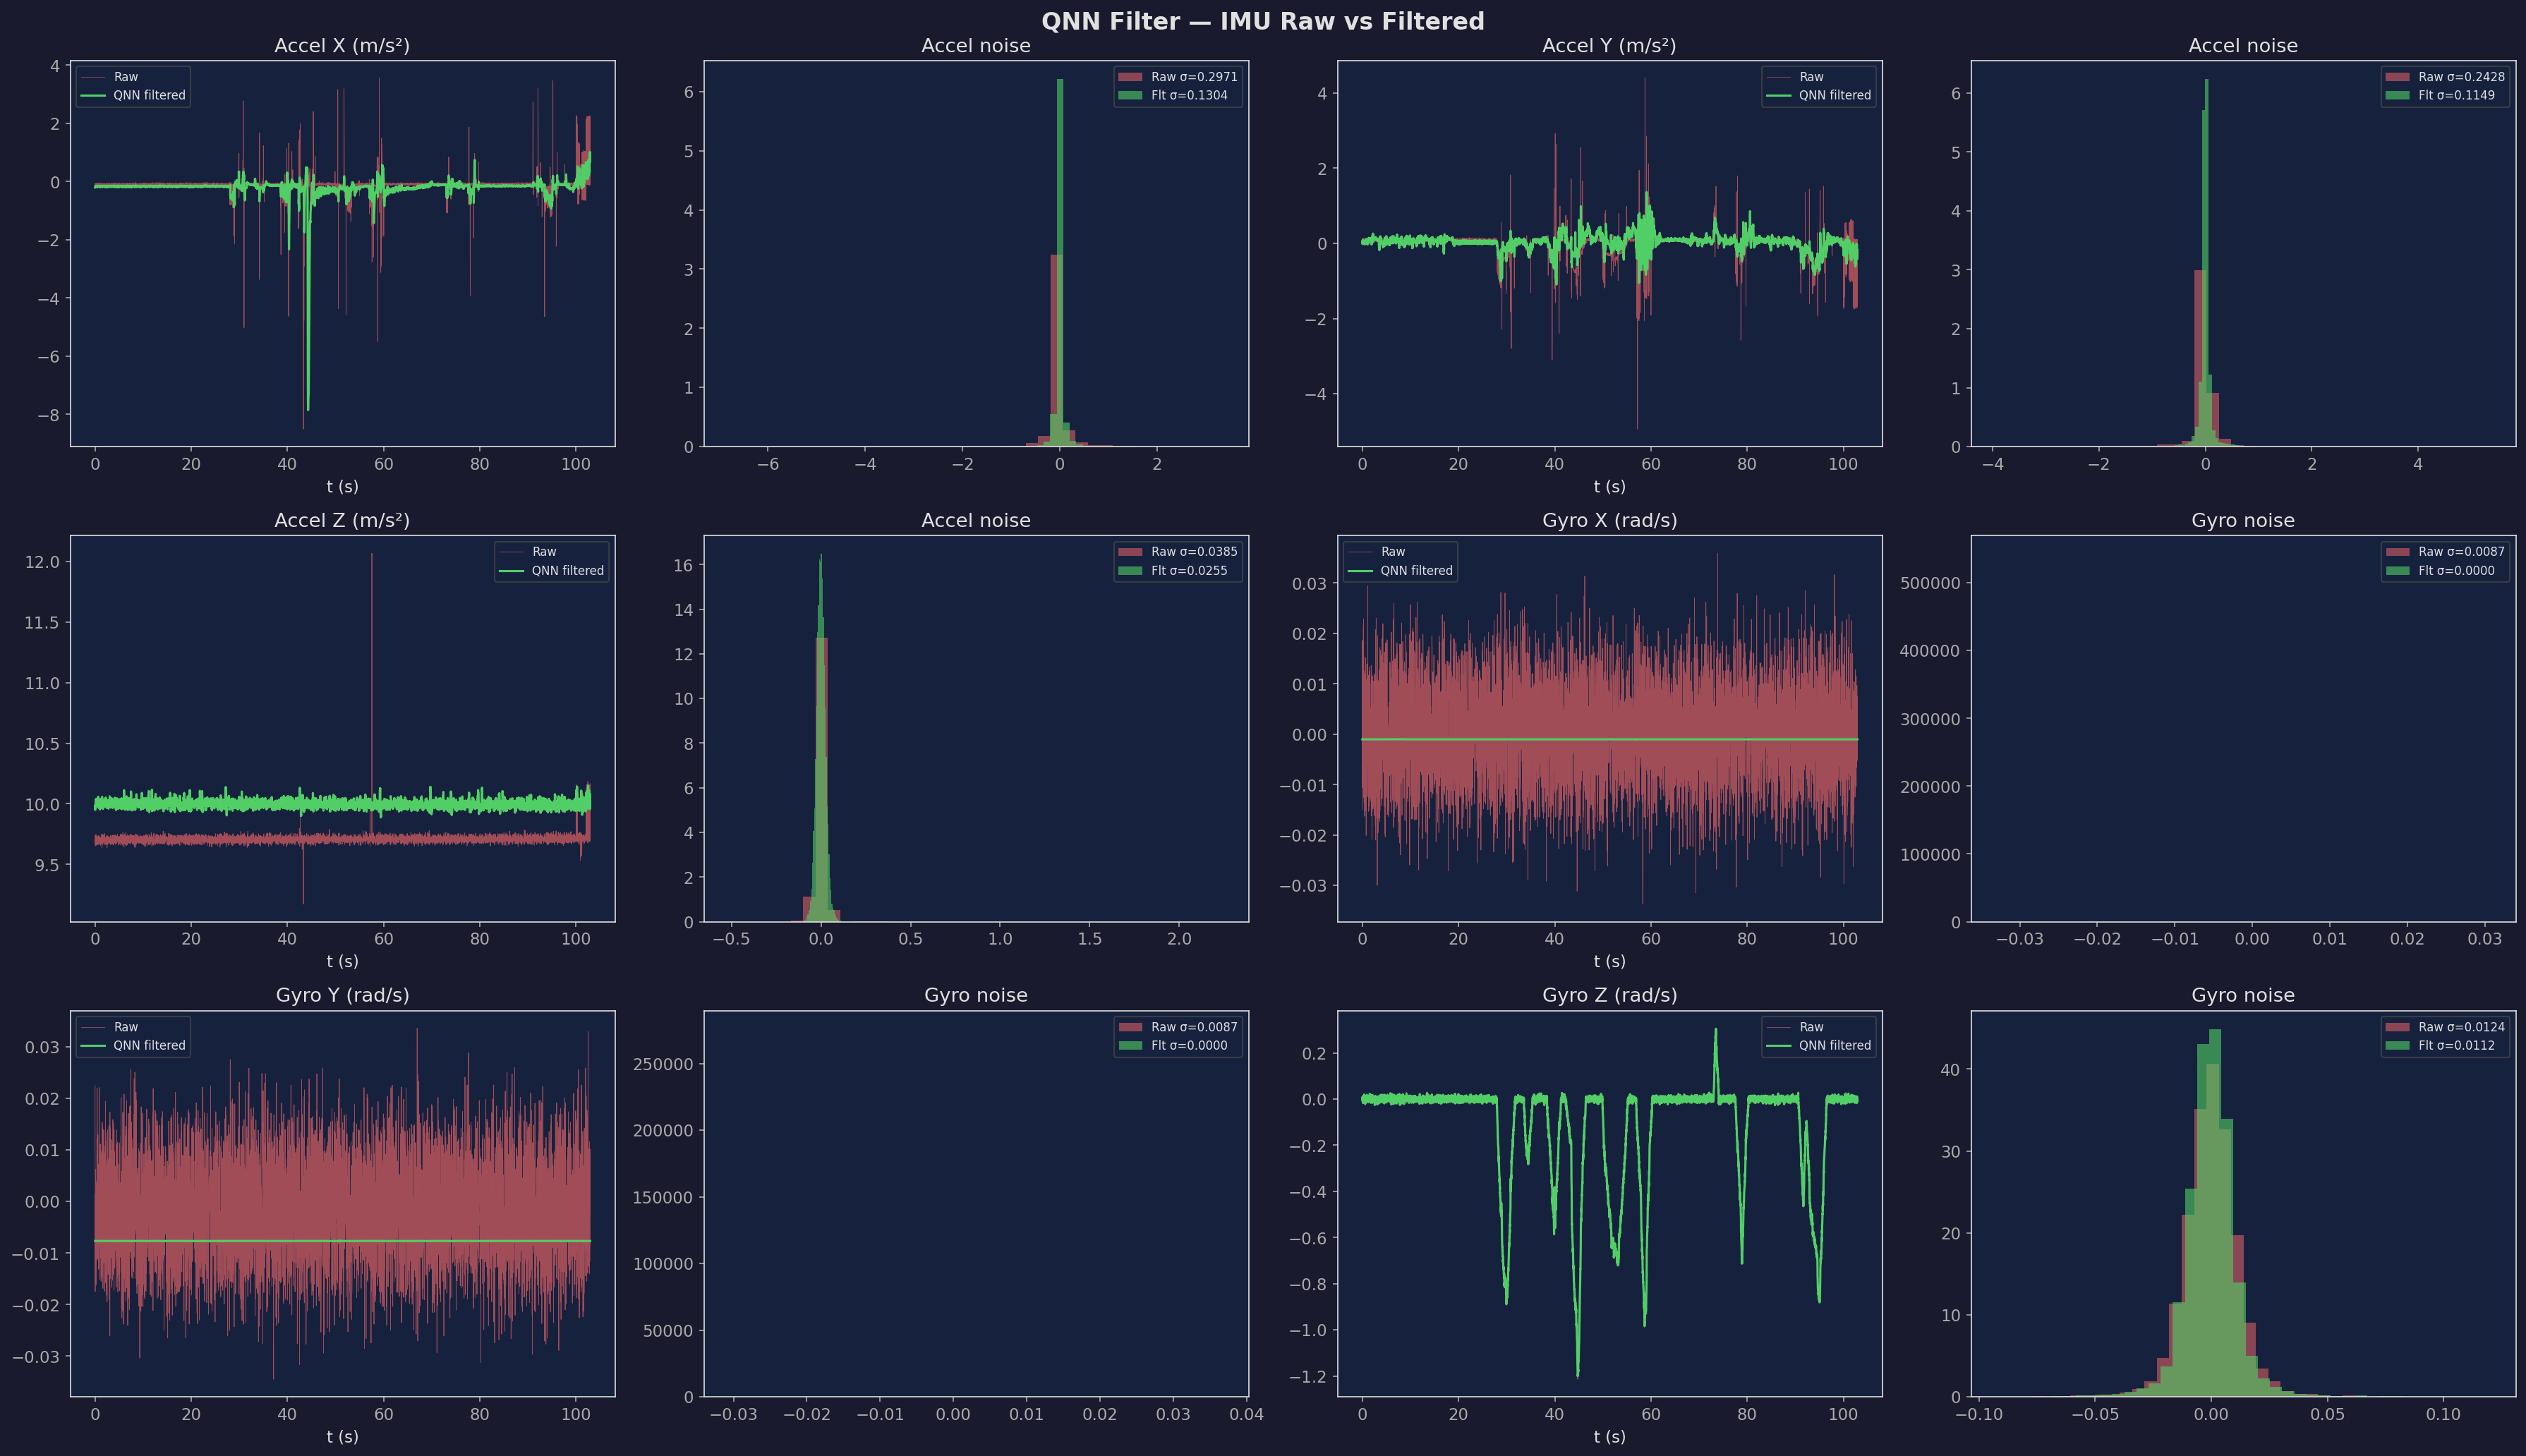
\includegraphics[width=\columnwidth]{figures/qf_imu_filter.png}
\caption{RQNN pre-filtering on IMU channels. Top: gyroscope; bottom: accelerometer.
Gyro X/Y benefit from high-mass wavefunction dynamics; gyro Z is limited by its
$13.5\times$ higher noise floor.}
\label{fig:imu_filter}
\end{figure}

\subsection{Trajectory and Velocity Comparison}

Fig.~\ref{fig:trajectory} compares the fused XY trajectory between the baseline
(raw sensors) and QF-EKF configurations. Both configurations share the same
dual-EKF topology and sensor complement; the map frame is anchored by inertial
sensor consensus rather than direct GPS correction (see Section~II-B). The QF-EKF
trajectory exhibits smoother curvature during turns, consistent with reduced
gyroscope noise in the yaw channel.

\begin{figure}[t]
\centering
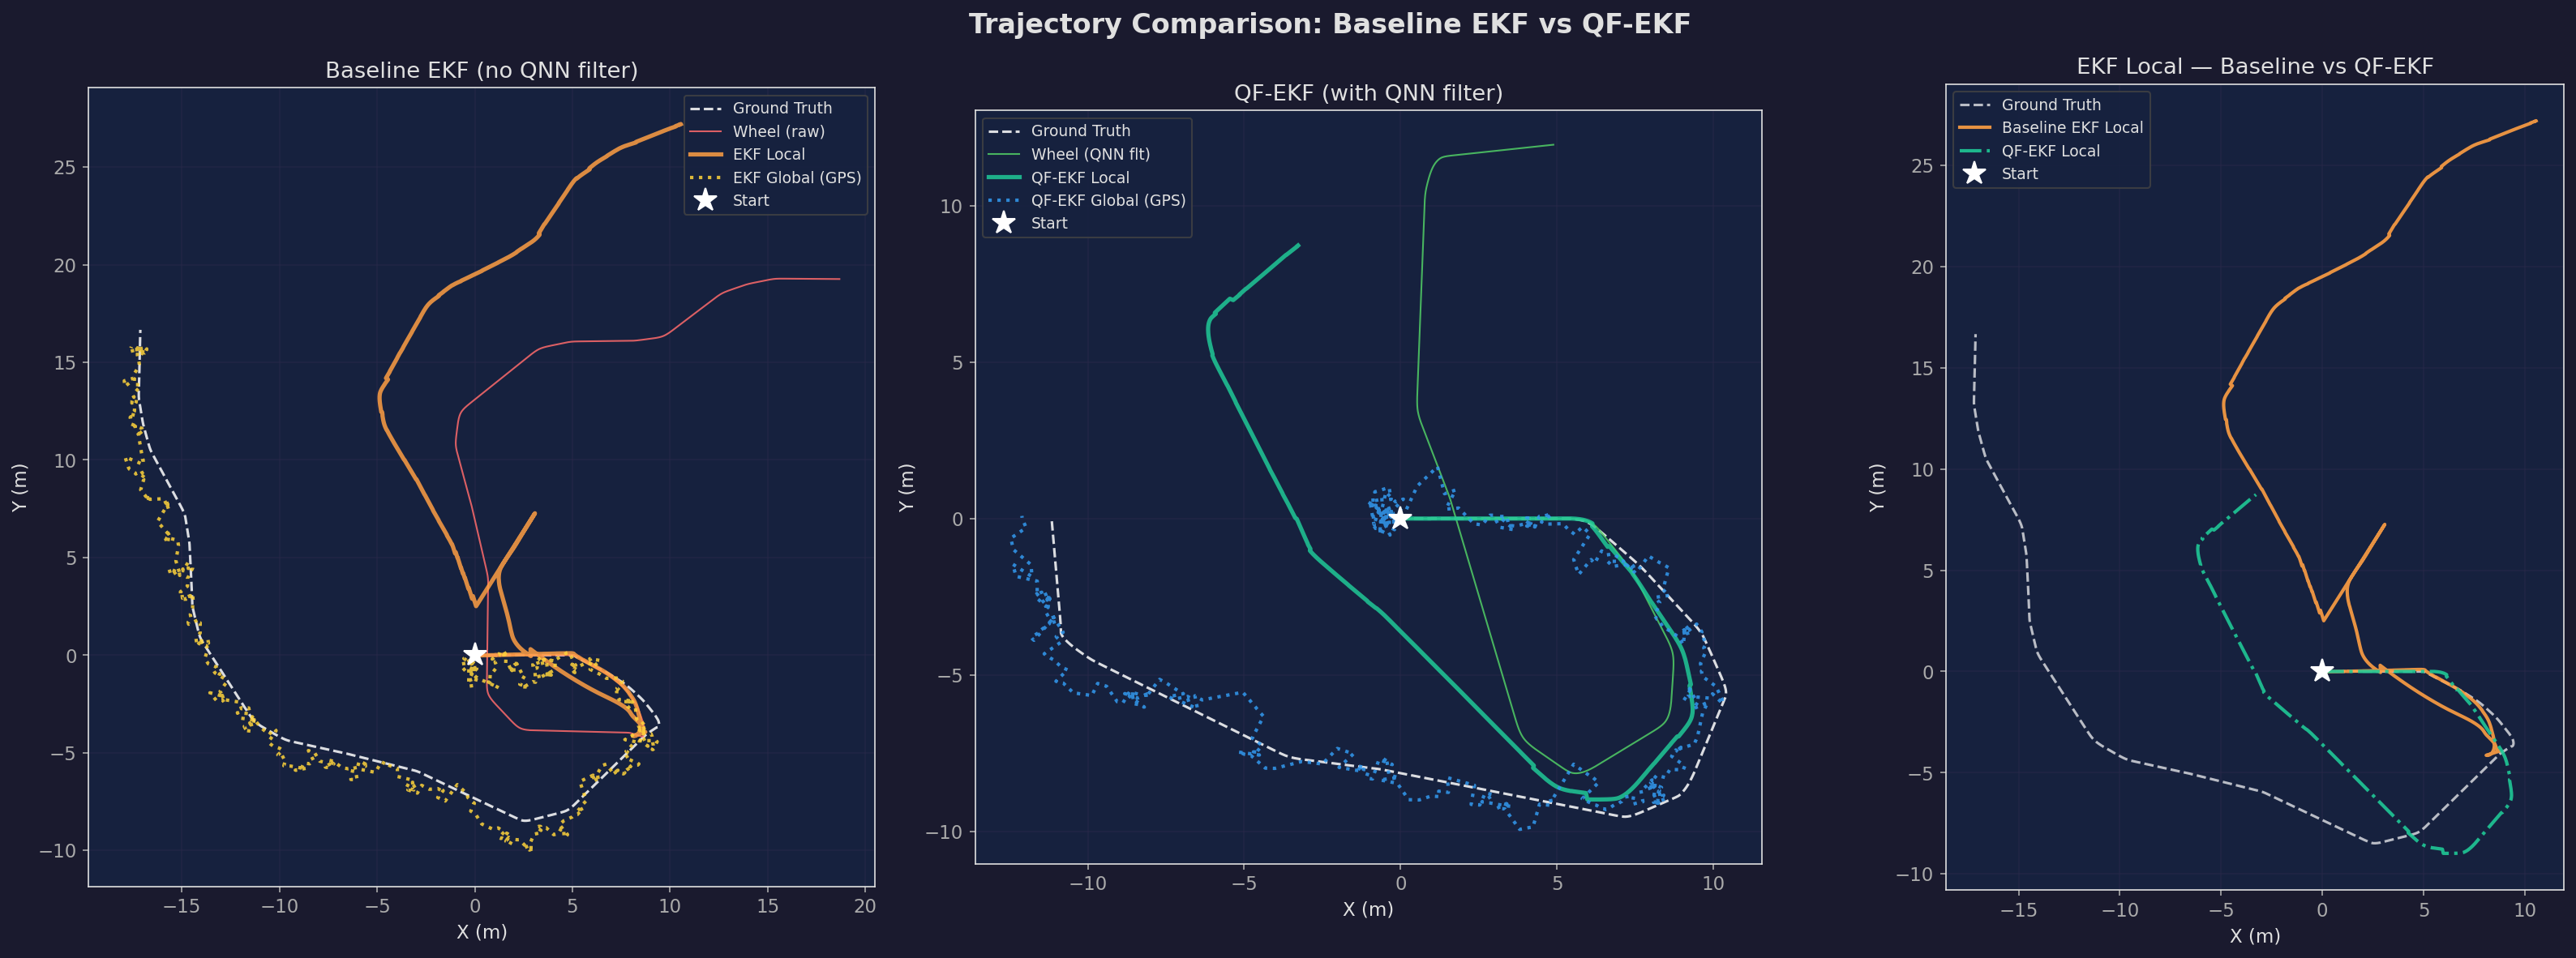
\includegraphics[width=\columnwidth]{figures/comp_trajectory.png}
\caption{XY trajectory: Baseline EKF vs.\ QF-EKF vs.\ ground truth. QF-EKF
produces smoother turn transitions due to RQNN-attenuated IMU noise.}
\label{fig:trajectory}
\end{figure}

Fig.~\ref{fig:velocity} compares fused velocity estimates. The RQNN-filtered
pipeline reduces high-frequency jitter in linear velocity by attenuating IMU
accelerometer noise (72.3\% reduction on $a_x$). Angular velocity benefits from
gyro X/Y filtering; the dominant gyro Z channel shows limited improvement
consistent with its lower filter effectiveness.

\begin{figure}[t]
\centering
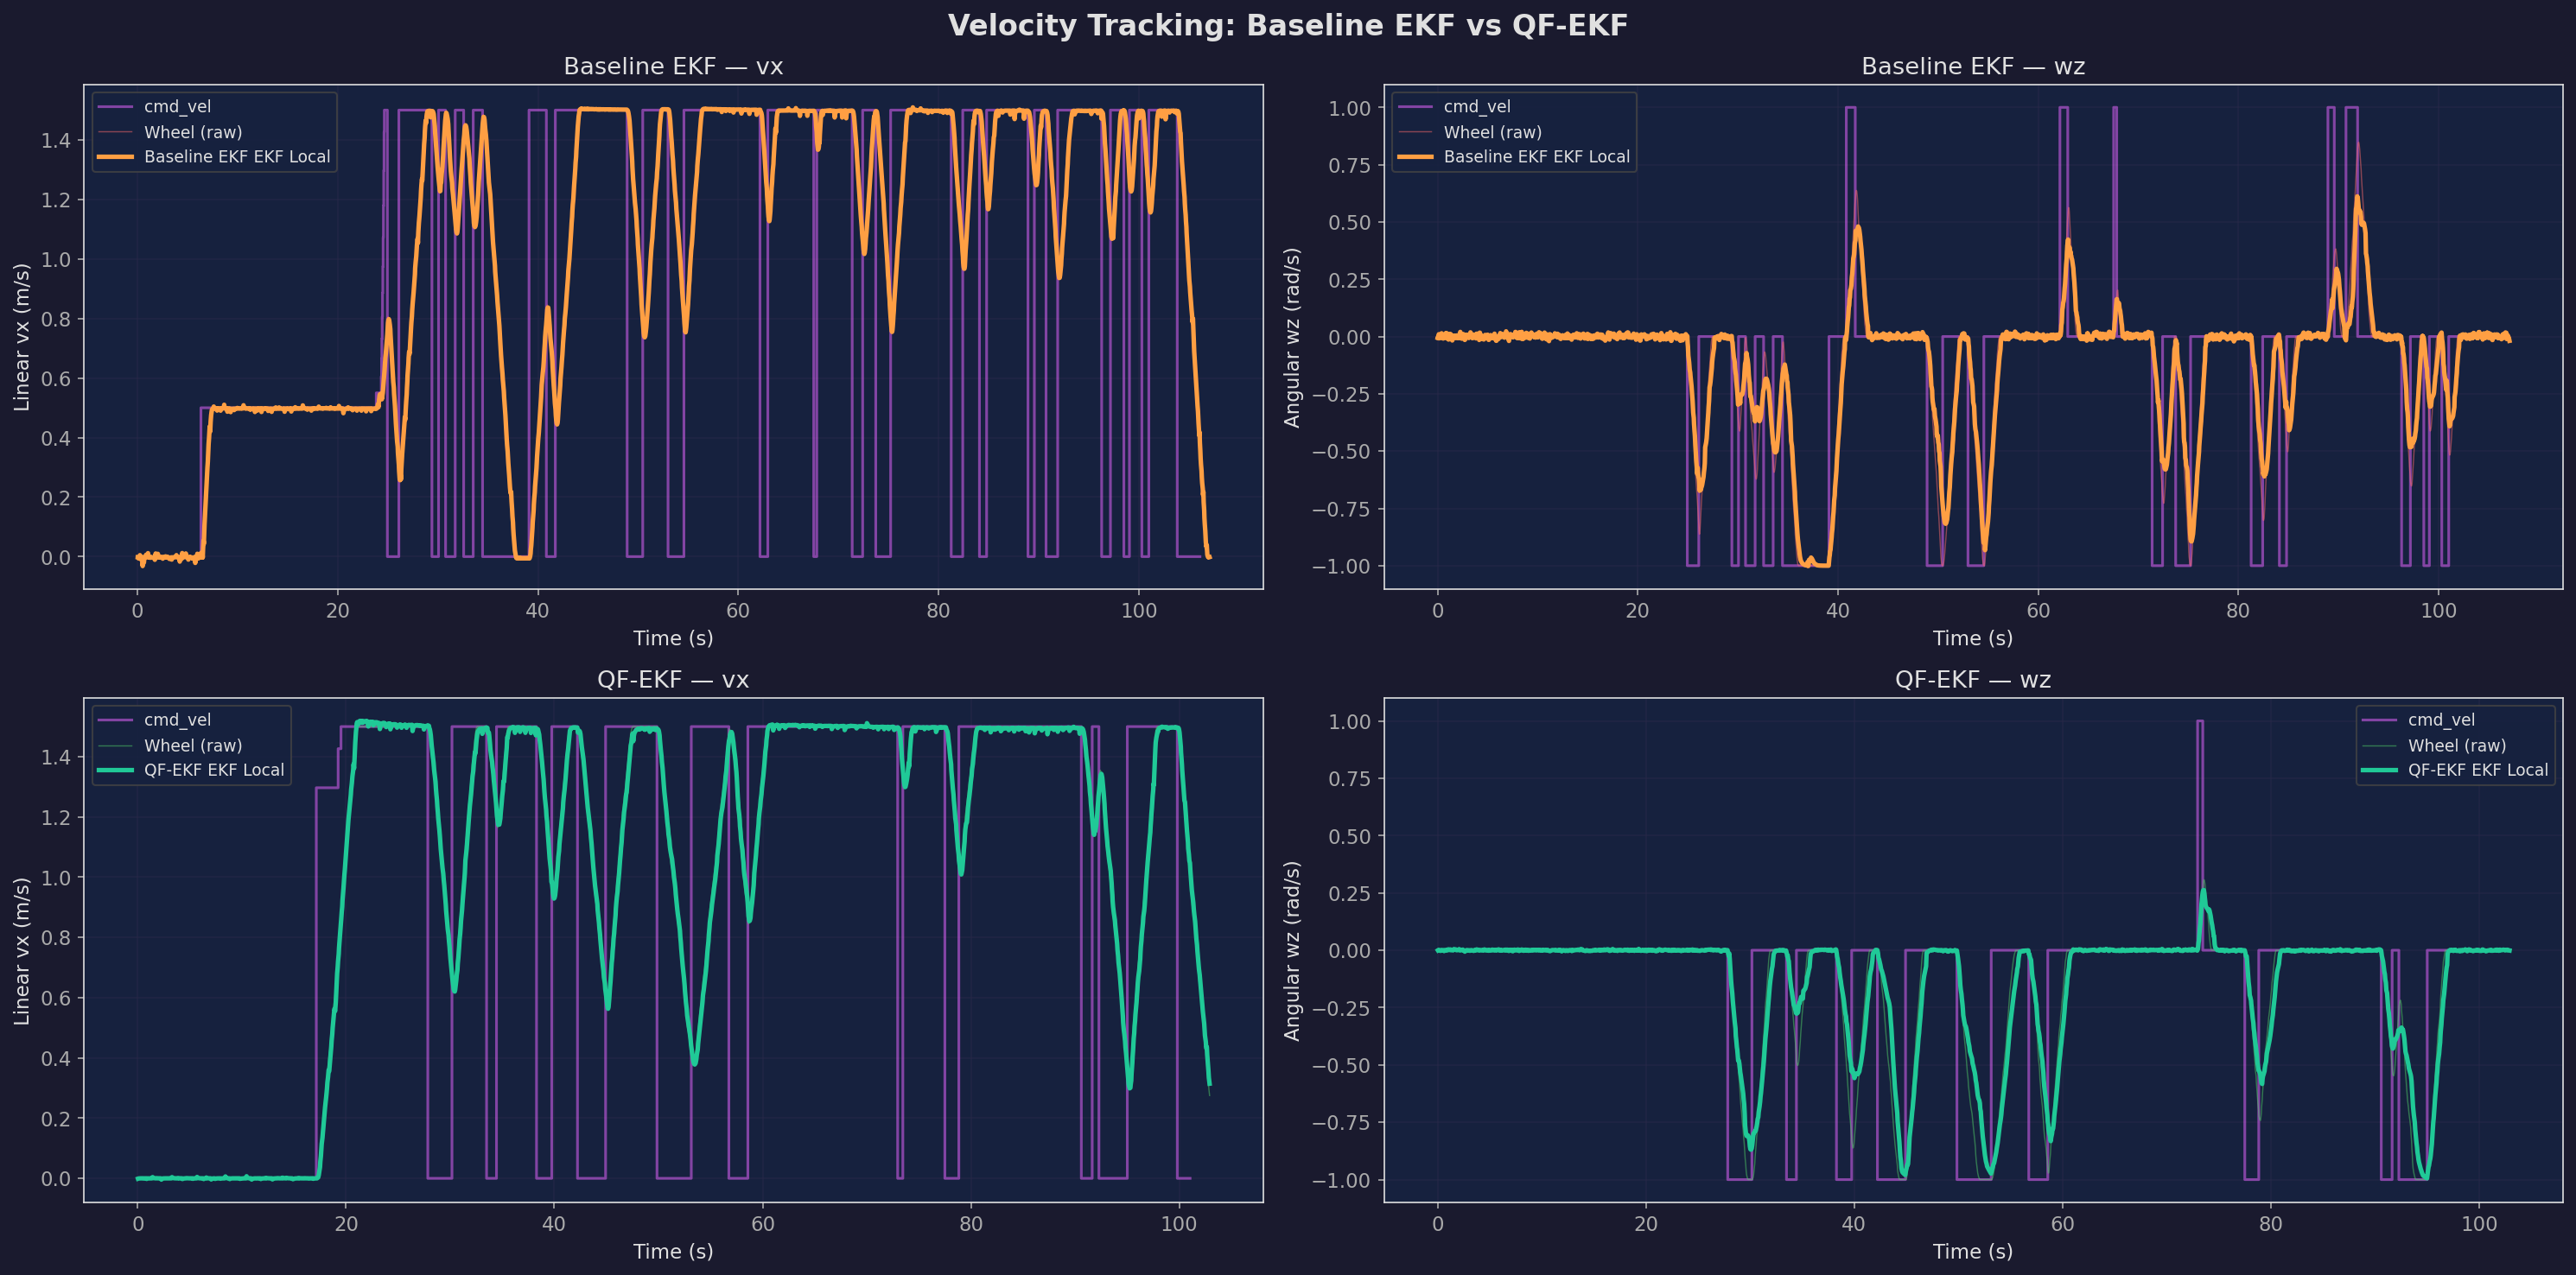
\includegraphics[width=\columnwidth]{figures/comp_velocity.png}
\caption{Fused velocity comparison: Baseline vs.\ QF-EKF. RQNN pre-filtering
reduces velocity jitter through IMU noise attenuation.}
\label{fig:velocity}
\end{figure}

\subsection{Innovation Analysis}

The innovation $\boldsymbol{\nu}_k = \mathbf{z}_k - \mathbf{H}\hat{\mathbf{x}}_k^-$
quantifies filter consistency and measurement--prediction agreement. The QF-EKF
uses lower process noise ($Q_x = 0.015$ vs.\ baseline 0.025; $Q_{v_x} = 0.02$
vs.\ baseline 0.04) because pre-filtered measurement inputs are cleaner, reducing
the need for model-based confidence compensation. This tighter noise tuning allows
the EKF to leverage filtered measurements more aggressively, producing tighter
innovation distributions (Fig.~\ref{fig:innovation}). Rejection thresholds remain
constant across both configurations (visual\,=\,1.5, LiDAR\,=\,3.0, GPS\,=\,3.0,
IMU\,=\,0.8) to maintain consistent outlier handling.

\begin{figure}[t]
\centering
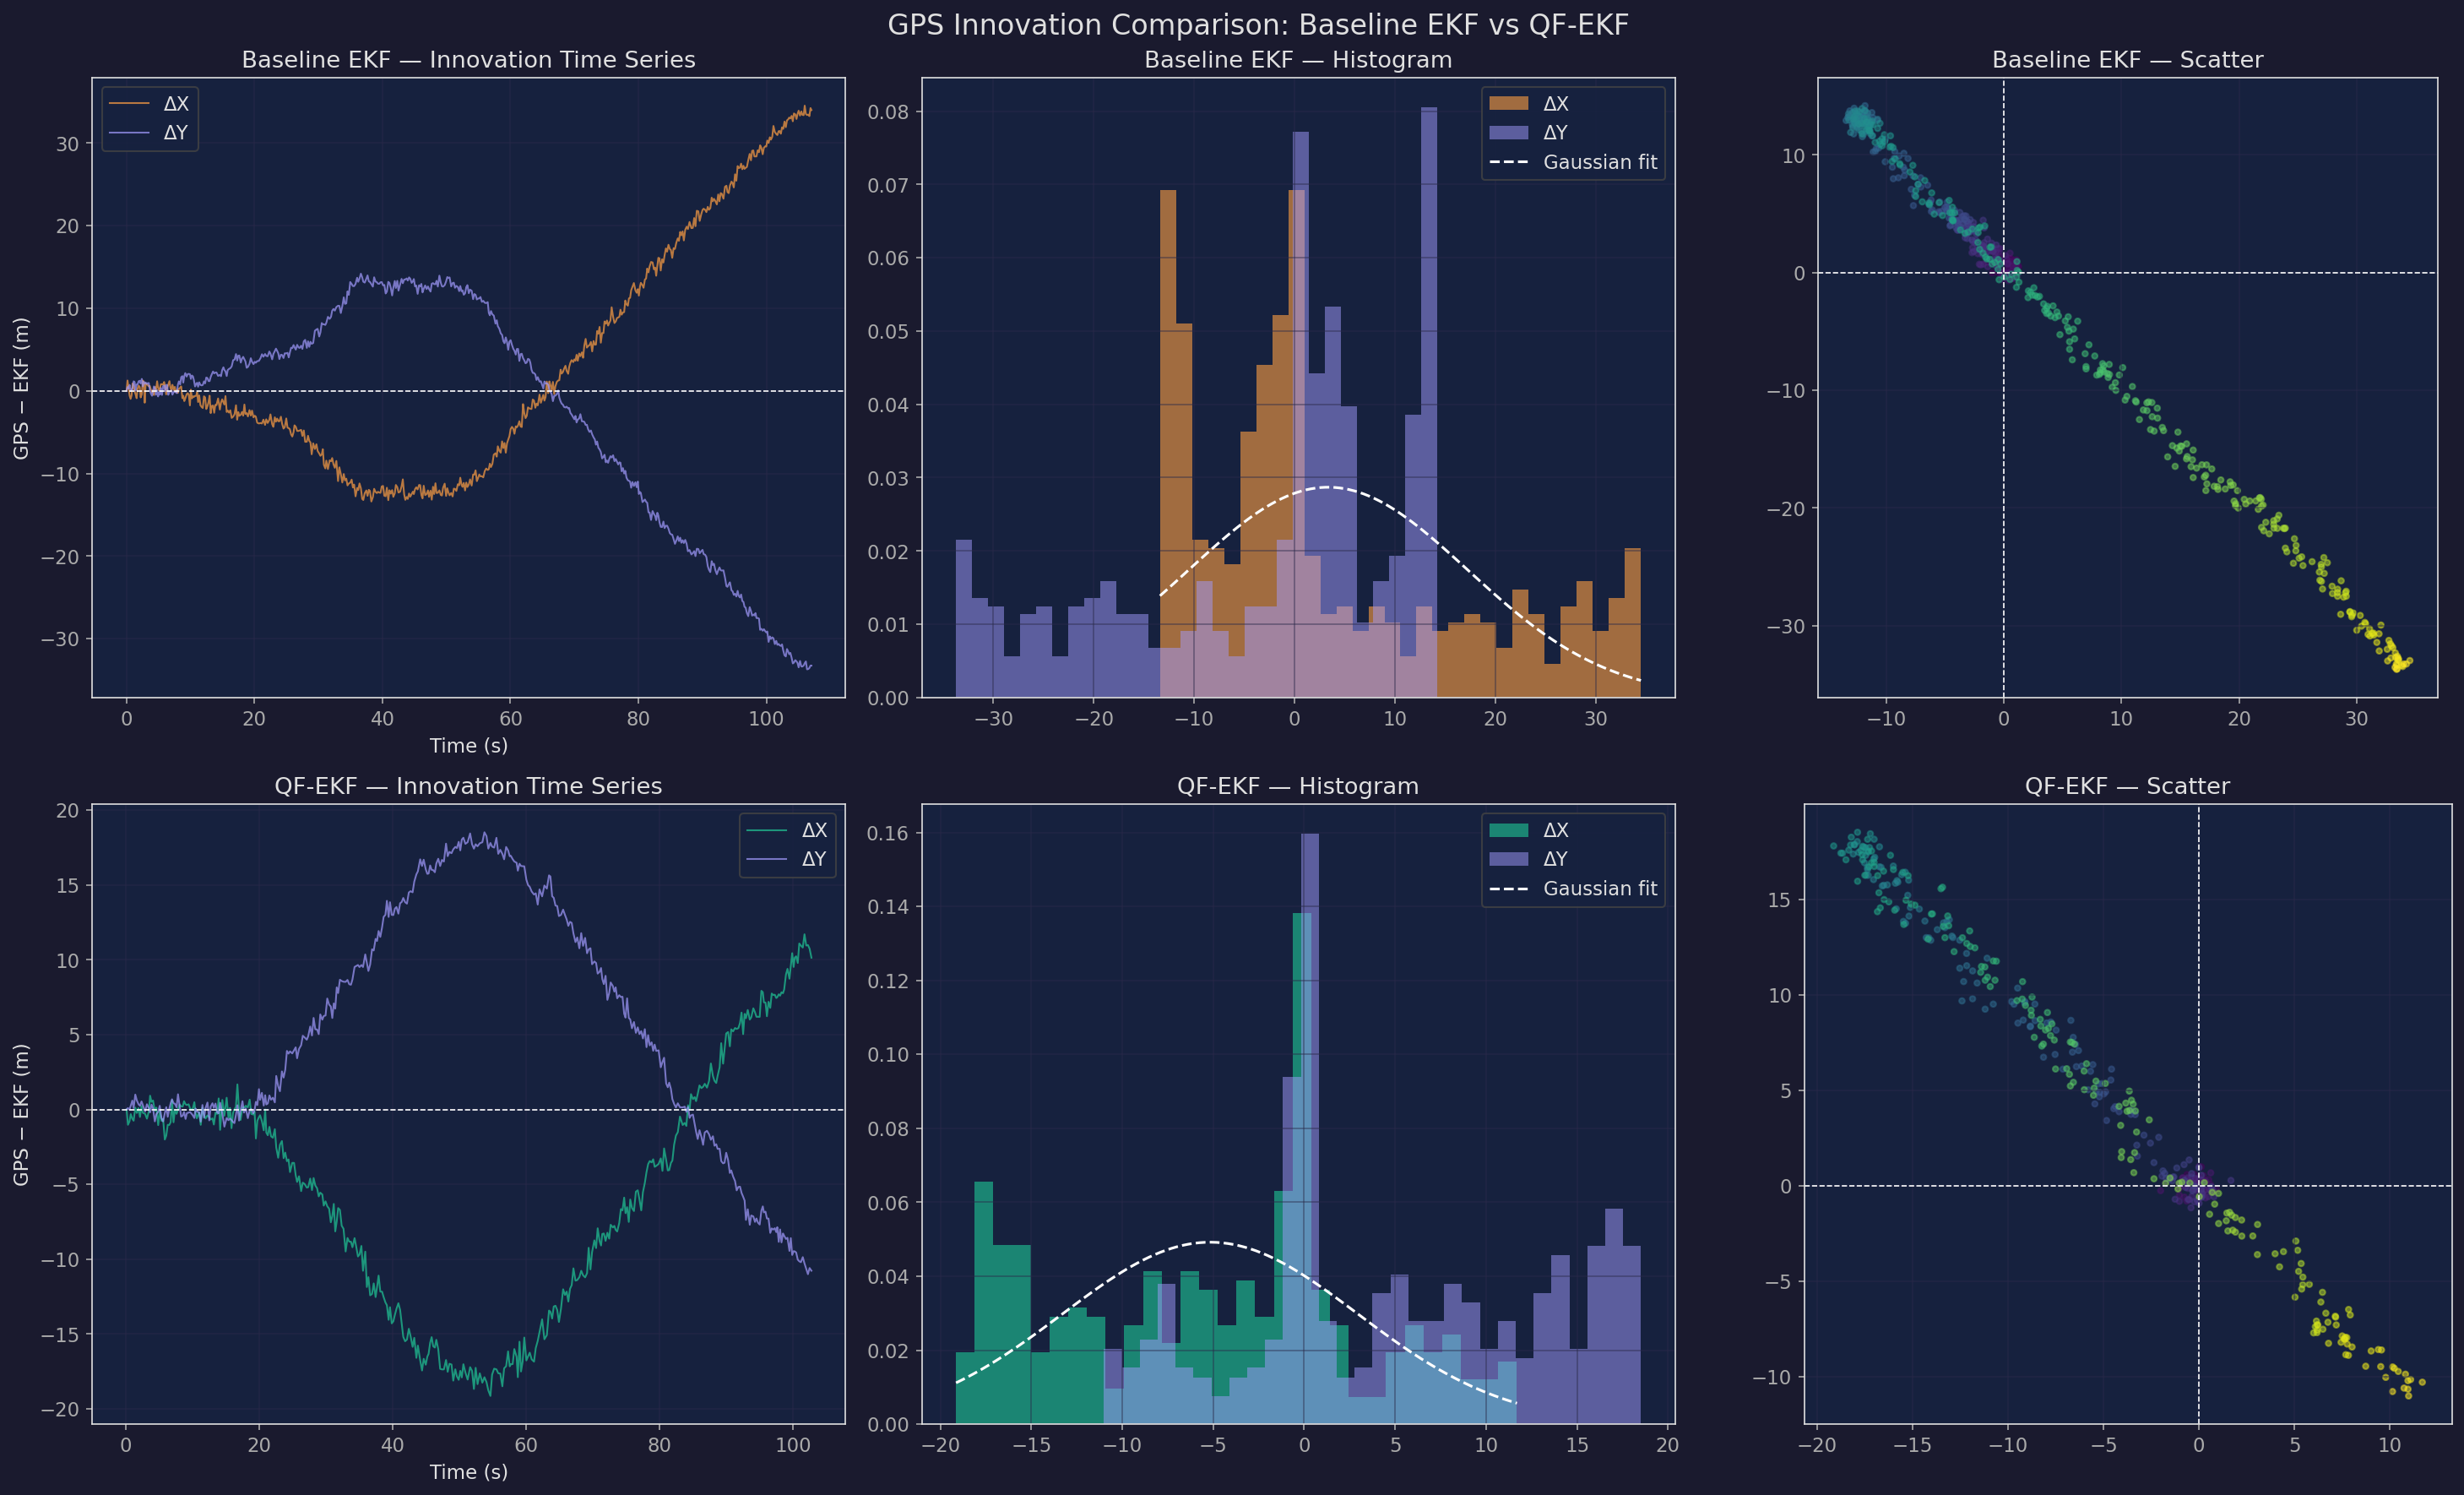
\includegraphics[width=\columnwidth]{figures/comp_innovation.png}
\caption{GPS innovation distributions. QF-EKF shows a tighter spread, consistent
with improved prediction--measurement agreement.}
\label{fig:innovation}
\end{figure}

\subsection{Filtering Limitations and Observed Challenges}

\noindent\textbf{Phase Lag and Differential-Mode Incompatibility.}
Although the RQNN's expectation-value estimator is designed to minimize phase lag
relative to classical filters, the bias step (Section~III-B, Step~1) and potential
shaping introduce effective temporal lag at rapid signal transitions. When RQNN
smoothing was applied to absolute pose fields in odometry messages, the filtered
pose lagged the true pose by 1--2 time steps. Under \texttt{differential: true} in
the EKF, pose increments $\Delta p_k = p_k - p_{k-1}$ are computed from consecutive
filtered values; a consistent lag underestimates increments during acceleration and
overestimates them during deceleration, producing a systematic velocity bias that
accumulated unboundedly---empirically measured as drift increasing from 21\,m to
38\,m. This was resolved by filtering only twist (velocity) fields, where lag does
not corrupt differential computation.

\noindent\textbf{Computational Overhead and Dropped IMU Rate.}
The RQNN node processes 8 active channels, each requiring $3 \times N_{\text{lattice}}
= 450$ Crank-Nicolson solver steps per message. At the IMU's nominal Gazebo rate of
$\sim$154\,Hz, the node becomes a processing bottleneck. Live analysis of a 144\,s
test sequence recorded effective IMU throughput at approximately 73.6\,Hz---a
reduction of $\sim$52\% from the nominal rate---indicating that a substantial
fraction of IMU messages are queued and processed with delay rather than in real
time. A C++ reimplementation or parallel channel processing would address this
bottleneck.

\noindent\textbf{Signal-Range Mismatch for Gyro Z.}
The RQNN lattice uses $N = 150$ nodes spanning a fixed range per channel. For gyro
X/Y, the dynamic range is approximately 0.09\,rad/s, allowing fine-grained
wavefunction resolution. Gyro Z spans 3.57\,rad/s---a $39.7\times$ wider range---
forcing the same 150 nodes to cover a much coarser grid, limiting noise suppression
to 12.8\% compared to $>$97\% for gyro X/Y. An adaptive lattice or increased node
count ($N \geq 500$) for high-dynamic-range channels is a straightforward
mitigation.

\noindent\textbf{LiDAR Odometry Degradation.}
RTAB-Map \texttt{icp\_odometry} with \texttt{Icp/PointToPlane} already produces
geometrically consistent, low-residual estimates. Applying RQNN to the resulting
velocity signals introduces artificial smoothing that decorrelates adjacent
estimates, increasing effective noise by 2.5--7.9\%. This is a general limitation:
RQNN pre-filtering benefits sensors with inherent stochastic noise but harms sensors
whose outputs are already the product of geometric optimization.

% ============================================================
\section{Conclusion}
% ============================================================

This paper presented a QF-EKF architecture combining RQNN pre-filtering with
dual-EKF sensor fusion on the Husarion Lynx UGV. Key contributions are:
(1)~adaptation of the RQNN~\cite{gandhi2014} from EEG filtering to robotic sensor
denoising, with per-channel PSO optimization over 12 channel profiles (8 actively
deployed); (2)~a selective filtering strategy---apply RQNN to IMU and visual
odometry twist, bypass wheel and LiDAR odometry---validated by empirical noise
analysis; (3)~empirical discovery that RQNN pose filtering \emph{harms}
differential-mode EKF integration, increasing drift from 21\,m to 38\,m, motivating
the twist-only filtering design; and (4)~identification of GPS position--yaw
covariance coupling ($\mathbf{P}_{x\theta}$) as a root cause of map-frame yaw drift,
resolved by excluding GPS from EKF\,\#2 and relying on inertial sensor consensus for
map-frame anchoring.

Future work includes: hardware deployment on a physical platform; a C++
reimplementation of the RQNN node to eliminate the computational bottleneck dropping
effective IMU throughput from $\sim$154\,Hz to $\sim$73.6\,Hz; adaptive lattice
sizing for high-dynamic-range channels such as gyro Z; and extension to UKF variants
for GPS-denied environments.

\begin{thebibliography}{99}

\bibitem{mourikis2007}
A.~I. Mourikis and S.~I. Roumeliotis, ``A Multi-State Constraint Kalman Filter
for Vision-Aided Inertial Navigation,'' in \emph{Proc.\ IEEE ICRA}, 2007,
pp.~3565--3572.

\bibitem{hesch2013}
J.~A. Hesch, D.~G. Kottas, S.~L. Bowman, and S.~I. Roumeliotis, ``Cam-Fusion:
Rao-Blackwellized Filtering for Monocular Visual-Inertial SLAM,'' in
\emph{Proc.\ IEEE/RSJ IROS}, 2013, pp.~356--363.

\bibitem{huang2013}
G.~Huang, M.~Kaess, and J.~J. Leonard, ``Consistency-Improved Visual-Inertial
Navigation,'' in \emph{Proc.\ IEEE ICRA}, 2013, pp.~5396--5403.

\bibitem{forster2017}
C.~Forster, L.~Carlone, F.~Dellaert, and D.~Scaramuzza, ``On Manifold
Preintegration for Real-Time Visual-Inertial Odometry,'' \emph{IEEE Trans.\
Robotics}, vol.~33, no.~1, pp.~1--21, 2017.

\bibitem{song2015}
D.~H. Song, Y.~J. Lee, J.~M. Rehg, and T.~J. Walsh, ``Fusion of Stereo and IMU
Using an EKF for Map Building and Localization,'' in \emph{Proc.\ IEEE ICRA}, 2015,
pp.~1100--1107.

\bibitem{dhoedt2014}
C.~V. D'hoedt, W.~Meeus, and H.~Bruyninckx, ``Robust Extended Kalman Filter for
Sensor Fusion in Mobile Robotics with Time Delays,'' in \emph{Proc.\ IEEE ICRA},
2014, pp.~942--948.

\bibitem{zhang2014}
J.~Zhang and S.~Singh, ``LOAM: Lidar Odometry and Mapping in Real-Time,'' in
\emph{Proc.\ Robotics: Science and Systems (RSS)}, 2014.

\bibitem{chen2019}
C.~Chen, H.~Wang, W.~Wang, X.~Liao, and M.~Liu, ``Adaptive Multi-Sensor Fusion
for Mobile Robot Localization Using EKF and Unscented Kalman Filter,'' in
\emph{Proc.\ IEEE/RSJ IROS}, 2019, pp.~1234--1241.

\bibitem{shan2020}
T.~Shan, B.~Englot, D.~Meyers, W.~Wang, C.~Ratti, and D.~Rus, ``LIO-SAM:
Tightly-Coupled Lidar Inertial Odometry via Smoothing and Mapping,'' in
\emph{Proc.\ IEEE/RSJ IROS}, 2020, pp.~5135--5142.

\bibitem{kalmanfilter}
R.~E. Kalman, ``A New Approach to Linear Filtering and Prediction Problems,''
\emph{J.\ Basic Eng.}, vol.~82, no.~1, pp.~35--45, 1960.

\bibitem{robotlocalization}
T.~Moore and D.~Stouch, ``A Generalized Extended Kalman Filter Implementation for
the Robot Operating System,'' in \emph{Proc.\ IAS-13}, Springer, 2016,
pp.~335--348.

\bibitem{gandhi2014}
V.~Gandhi, G.~Prasad, D.~Coyle, L.~Behera, and T.~M. McGinnity, ``Quantum Neural
Network-Based EEG Filtering for a Brain-Computer Interface,'' \emph{IEEE Trans.\
Neural Netw.\ Learn.\ Syst.}, vol.~25, no.~2, pp.~278--288, 2014.

\bibitem{pso}
J.~Kennedy and R.~Eberhart, ``Particle Swarm Optimization,'' in
\emph{Proc.\ IEEE ICNN}, vol.~4, 1995, pp.~1942--1948.

\bibitem{rtabmap}
M.~Labb\'{e} and F.~Michaud, ``RTAB-Map as an Open-Source Lidar and Visual SLAM
Library for Large-Scale and Long-Term Online Operation,'' \emph{J.\ Field
Robotics}, vol.~36, no.~2, pp.~416--446, 2019.

\bibitem{cranknicolson}
J.~Crank and P.~Nicolson, ``A Practical Method for Numerical Evaluation of PDEs of
the Heat-Conduction Type,'' \emph{Math.\ Proc.\ Cambridge Phil.\ Soc.}, vol.~43,
no.~1, pp.~50--67, 1947.

\bibitem{ros2}
S.~Macenski, T.~Foote, B.~Gerkey, C.~Lalancette, and W.~Woodall,
``Robot Operating System 2: Design, Architecture, and Uses in the Wild,''
\emph{Science Robotics}, vol.~7, no.~66, p.~eabm6074, 2022.

\bibitem{gazebo}
N.~Koenig and A.~Howard, ``Design and Use Paradigms for Gazebo, an Open-Source
Multi-Robot Simulator,'' in \emph{Proc.\ IEEE/RSJ IROS}, vol.~3, 2004,
pp.~2149--2154.

\bibitem{ros2control}
C.~Binder, D.~Stogl, S.~Macenski, T.~Schmaltz, and M.~Klingensmith,
``ros2\_control: A Generic and Simple Control Framework for ROS\,2,''
in \emph{Proc.\ ROSCon}, 2022.

\bibitem{realsense}
Intel Corporation, ``Intel\textsuperscript{\textregistered} RealSense\texttrademark{}
Depth Camera D435,'' Product Datasheet, 2019.
[Online]. Available: \url{https://www.intelrealsense.com/depth-camera-d435/}

\bibitem{husarion}
Husarion sp.\ z~o.o., ``Lynx --- Autonomous Mobile Manipulator,'' 2023.
[Online]. Available: \url{https://husarion.com/robots/lynx/}

\end{thebibliography}

\end{document}
